\chapter{Results} \label{ch:results}

{
\sloppy \raggedright
\section{Identification and characterisation of genome-wide binding sites of FOXM1 and FOXO3 using ChIP-seq analysis}
}

\subsection{Establishment of strategies for the ChIP-seq analysis of FOXM1 and FOXO3}

\begin{figure}[!ht]
    \centering
    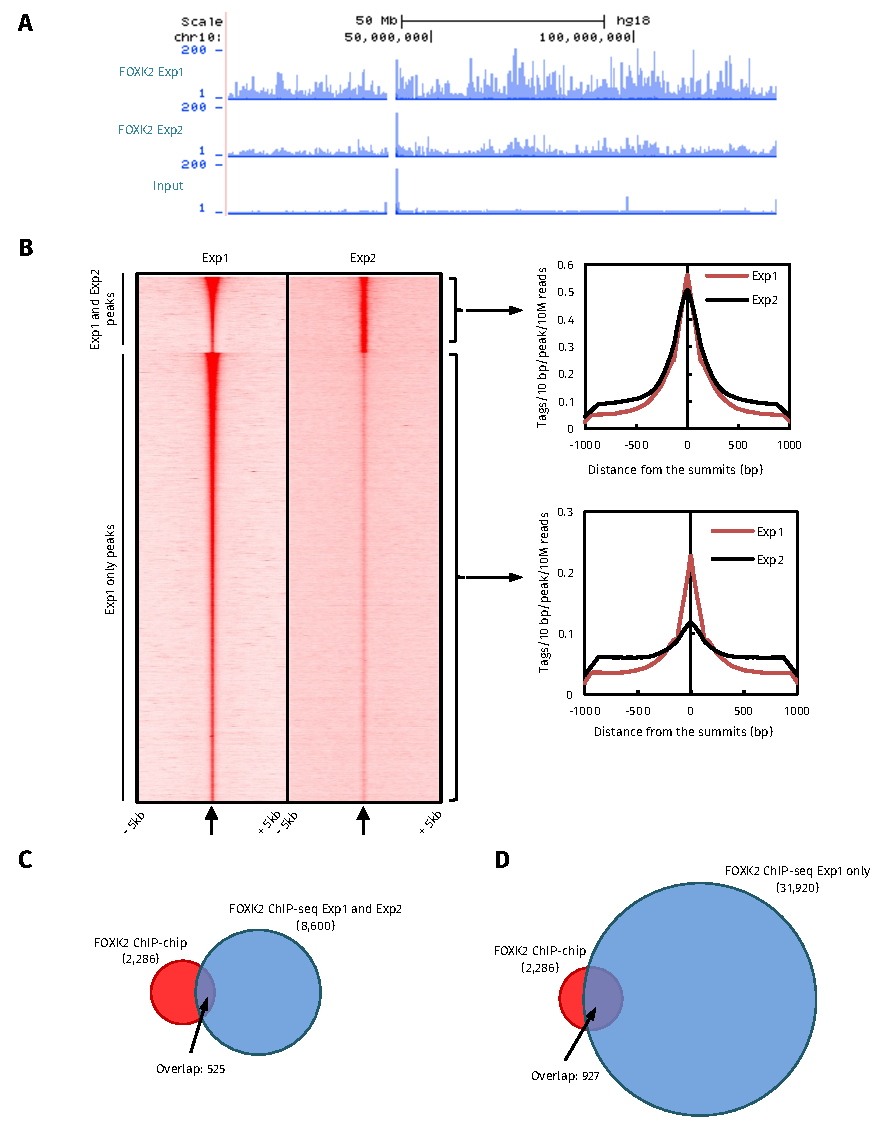
\includegraphics[width=0.9\textwidth]{chapter3/figures_overview/fig9.pdf}
    \caption[An overview of FOXK2 ChIP-seq data]{\textbf{An overview of FOXK2 ChIP-seq data. (A)} A snapshot of peak profiles of FOXK2 on the entire chromosome 10. Two ChIP experiments (indicated as Exp1 and Exp2) and one Input control are shown. \textbf{(B) Left,} heatmap of tag density profiles of the two FOXK2 ChIP-seq experiments around peaks that were identified from both experiments (Exp1 and Exp2 peaks), and peaks that were only identified from the first experiment (Exp1 only peaks). Tags were calculated in every 50 bp bin, and the density profiles were normalised to tags per 10 million total reads per bin. The middle point of each panel (indicated by small arrows below) represents the summit of the peak. 5 kb upstream and 5 kb downstream around the summit were plotted. \textbf{Right,} quantification of average of tags around the summit of Exp1 and Exp2 peaks and Exp1 only peaks. Peaks were aligned by their summits, and a region of -1 and +1 kb relative to the summit was selected. Tags were calculated in every 10 bp bin and normalised to tags per 10 million total reads per bin per peak. (\textbf{C} and \textbf{D}) Venn diagrams representing the overlaps in binding regions occupied by FOXK2 in ChIP-chip and ChIP-seq experiments. 8,600 Exp1and Exp2 peaks are shown in (\textbf{C}) and 31,920 peaks identified in the first experiment are shown in (\textbf{D}).}
    \label{fig:fig9}
\end{figure}

In order to investigate the \textit{in vivo} binding specificity of FOXM1, FOXO3 and FOXK2, it is necessary to interrogate the genome-wide binding profiles of the three Forkhead transcription factors. The ChIP-seq analysis of FOXK2 has already been done in proliferating U2OS cells by Dr. Zongling Ji in the Sharrocks lab (\cite{ji2012the}). Two independent experiments were performed, and 8,600 peaks were identified as present in both experiments. However, when comparing these two experiments, the first experiment turned out to be more sensitive than the second one based on the number of peaks detected, the peak height of the signal profile (for an example on chromosome 10, see \textbf{Figure \ref{fig:fig9}A}), and the average of signal intensity around the peaks (\textbf{Figure \ref{fig:fig9}B}). Previously, a ChIP-chip experiment of FOXK2 was also performed on Affymetrix Human Promoter 1.0R arrays. A total of 2,286 enriched binding regions were identified, and 525 (23\%) of them overlap with the 8,600 FOXK2 ChIP-seq peaks. When comparing to the first ChIP-seq experiment, the overlap of the ChIP-chip data increased to 927 (41\%) (\textbf{Figure \ref{fig:fig9}C}) (\cite{ji2012the}). In addition, some ChIP-qPCR validation also indicated that a lot of binding sites that only existed in the first experiment were true (\textbf{data not shown}). Therefore, in order to capture more FOXK2 binding events, we focused on the first FOXK2 ChIP-seq experiment in this study. In addition, to extract high confidence peaks from only one experiment, two peak callers MACS (\cite{zhang2008model-based}) and HOMER (\cite{heinz2010simple}) were used to call peaks. Only peaks that were called by both programs were kept. In this way, a total of 31,920 FOXK2 peaks were identified.

To investigate whether U2OS cells are suitable for studying the genome-wide binding events of FOXM1 and FOXO3, the expression of FOXM1 and FOXO3 were examined in this cell line. Early studies showed that protein levels of many cell cycle regulators (\textit{e.g.} several cyclins) undergo dramatic changes in different cell cycle stages (\cite{hochegger2008cyclin-dependent}). Since FOXM1 and FOXO3 have been linked to cell cycle regulation (\cite{alvarez2001forkhead,laoukili2005foxm1}), we first checked whether their protein levels were regulated during cell cycle. U2OS cells were synchronised at G1/S boundary by double thymidine block, and the cell lysates were collected at different time points after release from the block, followed by flow cytometry analysis for cell cycle profile or western blot analysis for protein expression. Two major bands and multiple closely-positioned bands with different mobility were observed after probing with a FOXM1 antibody and a FOXO3 antibody, respectively (\textbf{Figure \ref{fig:fig10}A}). To determine which bands corresponded to FOXM1 and FOXO3 protein rather than non-specific binding of the antibodies to other proteins, western blot analyses were performed after the transfection of a non-targeting control siRNA and siRNAs against either \textit{FOXM1} or \textit{FOXO3}. In the case of FOXM1, the two major bands disappeared after the knockdown, indicating that both bands are FOXM1 protein (\textbf{Figure \ref{fig:fig10}B}, left panel). In the case of FOXO3, most bands were reduced to background level after knockdown except one upper band, indicating a non-specific band recognised by this antibody (\textbf{Figure \ref{fig:fig10}B}, right panel). After treating the cell lysate with lambda phosphatase, both FOXM1 and FOXO3 exhibited a single uniform motility band (data not shown and \cite{park2008anaphase-promoting}), which demonstrate that the differences of mobility of the proteins are due to phosphorylation.

The protein level of FOXO3 stayed relatively constant throughout the cell cycle (\textbf{Figure \ref{fig:fig10}A}, middle panel). However, both phosphorylation and expression of FOXM1 oscillated during the cell cycle, with a low level at G1 phase (\textbf{Figure \ref{fig:fig10}A}, lane 2) and the highest level as cells accumulate at G2 and M phase (\textbf{Figure \ref{fig:fig10}A}, lane 5).

\begin{figure}[h]
    \centering
    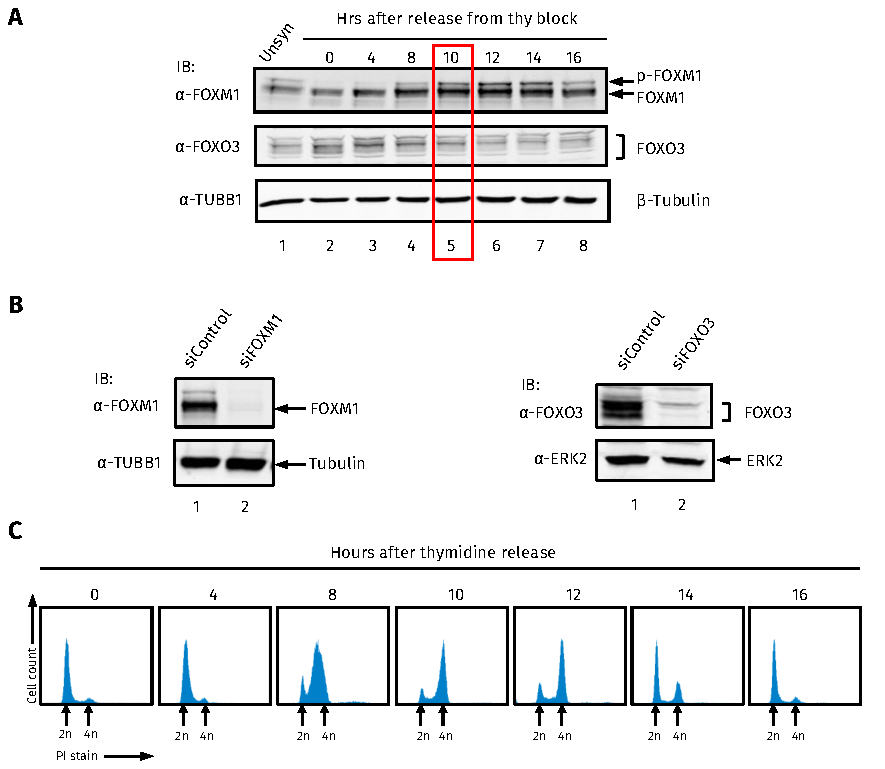
\includegraphics[width=0.9\textwidth]{chapter3/figures_overview/fig10.pdf}
    \caption[The expression of FOXM1 and FOXO3 in different cell cycle stages]{\textbf{The expression of FOXM1 and FOXO3 in different cell cycle stages. (A)} U2OS cell were synchronised at the G1/S boundary using double thymidine block and released into fresh media. Cells were collected at different time points as indicated after the release from double thymidine (thy) block. Total cell lysates were immunoblotted (IB) with the indicated antibodies to check the expression of endogenous FOXM1, FOXO3, and TUBB1 ($\beta$-Tubulin, as a loading control). Unsynchronised cells (Unsyn) are shown in lane 1. The positions of the bands corresponding to FOXM1/FOXO3 and the phosphorylated form of FOXM1 (p-FOXM1) are indicated. The red rectangle highlights the time point that was used for ChIP-seq experiments of FOXM1. \textbf{(B)} U2OS cells were transfected with a non-targeting control siRNA and siRNAs against either \textit{FOXM1} or \textit{FOXO3}. 48 hours after transfection, cell lysates were collected and immunoblotted with the indicated antibodies. TUBB1 and ERK2 were used as loading controls. \textbf{(C)} Flow cytometry analyses of the DNA content by propidium iodide (PI) staining of U2OS cells at different time points after the release from double thymidine block. The DNA content of diploid cells (2n) and tetraploid cells (4n) are indicated.}
    \label{fig:fig10}
\end{figure}

It is generally believed that protein abundance is an important factor that will influence ChIP-seq results (\cite{kidder2011chip-seq:}). Therefore, in order to maximise the chance of identifying the binding events, FOXM1 ChIP-seq analysis was performed in U2OS cells which were in the G2 and M phases of the cell cycle, \textit{i.e.} 10 hours after release from a double thymidine block (\textbf{Figure \ref{fig:fig10}A}, lane 5 and \textbf{Figure \ref{fig:fig10}C}), using a FOXM1 antibody.

\begin{figure}[!h]
    \centering
    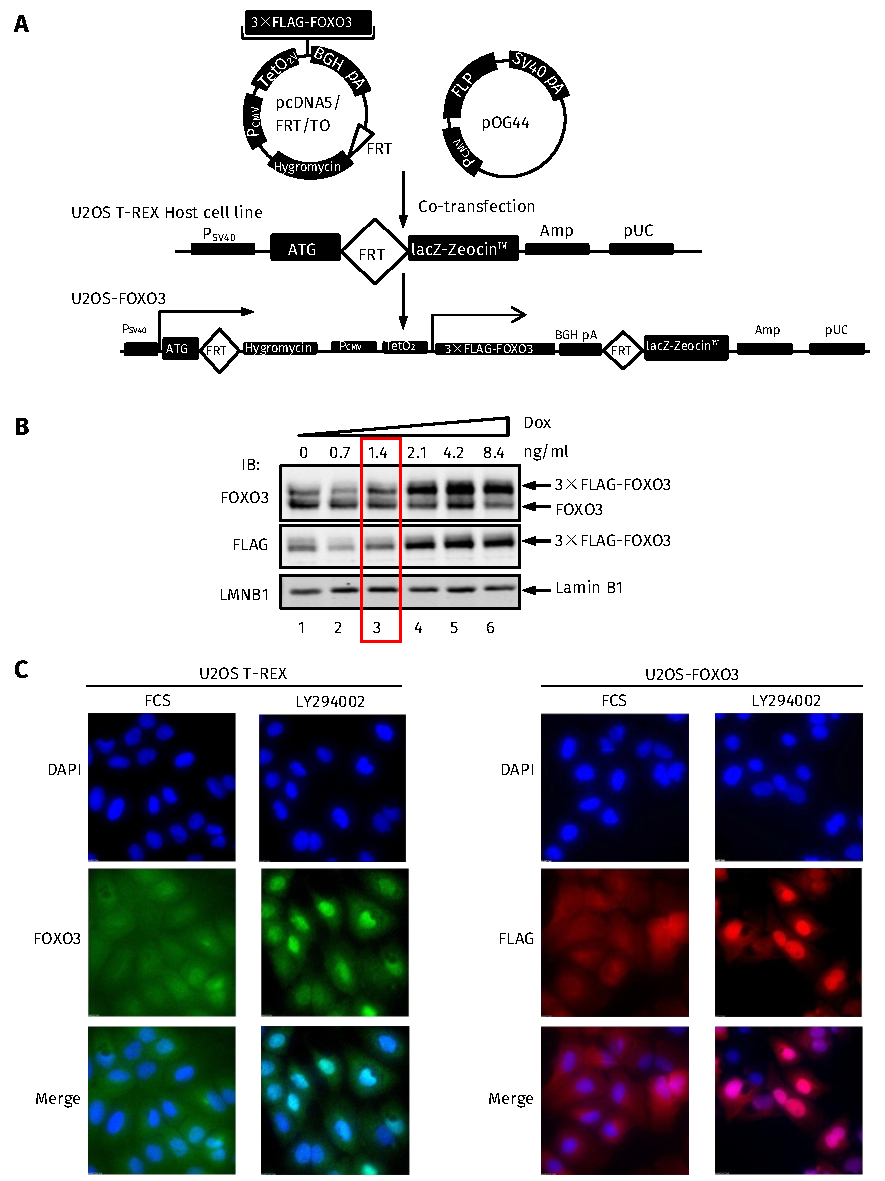
\includegraphics[width=0.9\textwidth]{chapter3/figures_overview/fig11.pdf}
    \caption[Establishment of 3$\times$FLAG-FOXO3 stable cell line]{\textbf{Establishment of 3$\times$FLAG-FOXO3 stable cell line. (A)} Schematic view of the strategy for constructing the 3$\times$FLAG-FOXO3 plasmid and the U2OS-FOXO3 stable cell line. \textbf{(B)} Varying concentrations of doxycycline (Dox) were added to culture media to induce the expression of the transgene. 24 hours after treatment, protein expression was examined by immunoblotting with different antibodies as indicated. LMNB1 (Lamin B1) was used as loading control. The positions of endogenous FOXO3 and 3$\times$FLAG-FOXO3 were indicated. The red rectangle indicates the concentration of doxycycline used for treating cells prior to ChIP. \textbf{(C)} Immunofluorescence analysis of endogenous FOXO3 and 3$\times$FLAG-FOXO3 cellular localisation in the U2OS T-REX host cell line and U2OS-FOXO3 stable cell line, respectively. The U2OS T-REX host cell line was stained with FOXO3 (75D8) antibody (\textit{i.e.} endogenous FOXO3; green) and DAPI; The U2OS-FOXO3 stable cell line was stained with FLAG antibody (\textit{i.e.} 3$\times$FLAG-FOXO3; red) and DAPI. Where indicated, cells were treated with 20 $\mu$M LY294002 or maintained in media containing FCS without this inhibitor.}
    \label{fig:fig11}
\end{figure}

Due to the lack of a suitable ChIP-grade antibody for FOXO3, a triple FLAG epitope tag was introduced to the N-terminus of FOXO3 (3$\times$FLAG-FOXO3) and cloned into the pcDNA5/FRT/TO vector (\textbf{Figure \ref{fig:fig11}A}). In this vector, the expression of 3$\times$FLAG-FOXO3 is driven by a tetracycline-inducible CMV promoter. The pcDNA5/FRT/TO/3$\times$FLAG-FOXO3 construct was co-transfected with the pOG44 vector, which encodes the Flp recombinase, into the Flip-In\sus{TM} U2OS host cell line that stably expresses the Tet repressor and contains a single integrated FRT site. After the co-transfection, the stable cell line (U2OS-FOXO3) was generated by maintaining the cells in the appropriate selection markers. By this approach, the U2OS-FOXO3 stable cell line was obtained which has only one single copy of the 3$\times$FLAG-FOXO3 transgene integrated into the specific locus in the genome, and the expression of the transgene can be controlled by adding varying concentrations of tetracycline/doxycycline (\textbf{Figure \ref{fig:fig11}A}). To examine the expression of 3$\times$FLAG-FOXO3 in response to doxycycline, different amounts of doxycycline were added to induce the expression of the transgene for 24 hours (18 hours after induction, the expression of 3$\times$FLAG-FOXO3 already became saturated, data not shown). Under normal cell culture condition (\textit{i.e.} DMEM with 10\% FCS) and without adding any doxycycline, there was some basal expression of 3$\times$FLAG-FOXO3 (\enquote{leaky} expression) due to the presence of tetracycline in the FCS (\textbf{Figure \ref{fig:fig11}B}, lane 1). The expression of 3$\times$FLAG-FOXO3 went up in line with the increase of the concentration of doxycycline added, and its level reached saturation when the concentration of doxycycline was at 4.2 ng/mL (\textbf{Figure \ref{fig:fig11}B}, lane 5).

Previous studies have shown that the nuclear localisation of FOXO3 is tightly controlled by PI3K/AKT signalling. Phosphorylation of FOXO3 by AKT results in its nuclear export through the interaction with 14-3-3 protein, and inhibition of PI3K/AKT signalling causes FOXO3 to enter the nucleus (\cite{brunet1999akt}). To check that the epitope-tagged FOXO3 behaves in the same way as the endogenous FOXO3, the localisation of the 3$\times$FLAG-FOXO3 was examined by immunofluorescence with or without LY294002, a specific inhibitor of PI3 kinase. As expected, under normal cell culture condition (in the presence of FCS), the endogenous FOXO3 is dispersed throughout the cytoplasm and the nucleus. After treatment with LY294002, most FOXO3 was relocated into the nucleus (\textbf{Figure \ref{fig:fig11}C}, left panel). Similarly, 3$\times$FLAG-FOXO3 spread out between the cytoplasm and the nucleus in the presence of FCS, and was predominantly located in the nucleus after addition of LY294002 (\textbf{Figure \ref{fig:fig11}C}, right panel). This demonstrates that the FLAG tagged FOXO3 transgene behaves in a similar manner to endogenous FOXO3.

Therefore, to investigate the genome-wide binding events of FOXO3, doxycycline was added at a concentration of 1.4 ng/mL which induced 3$\times$FLAG-FOXO3 expression to a level that is comparable to the endogenous FOXO3 (\textbf{Figure \ref{fig:fig11}B}, lane 3). A ChIP-seq experiment was performed under these conditions on U2OS-FOXO3 stable cell line using a FLAG antibody after 24 hours treatment with LY294002. In the meantime, a control ChIP experiment was also performed on U2OS T-REX host cell line which does not express the 3$\times$FLAG-FOXO3 transgene using the same antibody.

In summary, both FOXM1 and FOXO3 are expressed in U2OS cells, indicating this cell line is suitable for studying the genome-wide binding events of these two factors. The strategies for performing ChIP-seq experiments for FOXM1 and FOXO3 have been successfully established.

\subsection{Genome-wide chromatin-binding landscapes of Forkhead transcription factors}

Two biological replicates were performed for FOXM1 ChIP-seq experiments, yielding 27,892,797 and 8,906,067 uniquely mapped reads. MACS was used to call peaks, and a total of 270 peaks which were called from both experiments were identified as high confidence FOXM1 peaks. Although the sequencing depth of the second replicate was lower than the first one, the average peak signals of the second experiment was higher than the first one (\textbf{Figure \ref{fig:fig12}A}). In addition, quantitative comparison between the signal intensities from the two replicates showed that the two experiments have good correlation ($r=0.82$, Pearson correlation coefficient) (\textbf{Figure \ref{fig:fig12}B}), suggesting that the qualities of the two replicates around these peaks were similar.

Only one experiment was performed for FOXO3 ChIP-seq, yielding 38,149,670 mappable reads. In order to get high confidence peaks from one experiment, the same method which was used to extract FOXK2 peaks was applied to the FOXO3 ChIP-seq data. By the use of MACS and HOMER, a total of 6,089 peaks which were called by both programs were preserved as high confidence FOXO3 peaks.

The numbers of binding sites were vastly different among these three factors. This became apparent by looking at the peak profile across chromosomes as illustrated from the chromosome 1 (\textbf{Figure \ref{fig:fig13}A} and \textbf{B}). In particular, the small number of FOXM1 peaks is significantly less than commonly-observed number of peaks for other human transcription factors in cell culture systems (reviewed in \cite{macquarrie2011genome-wide}).

\begin{figure}[!h]
    \centering
    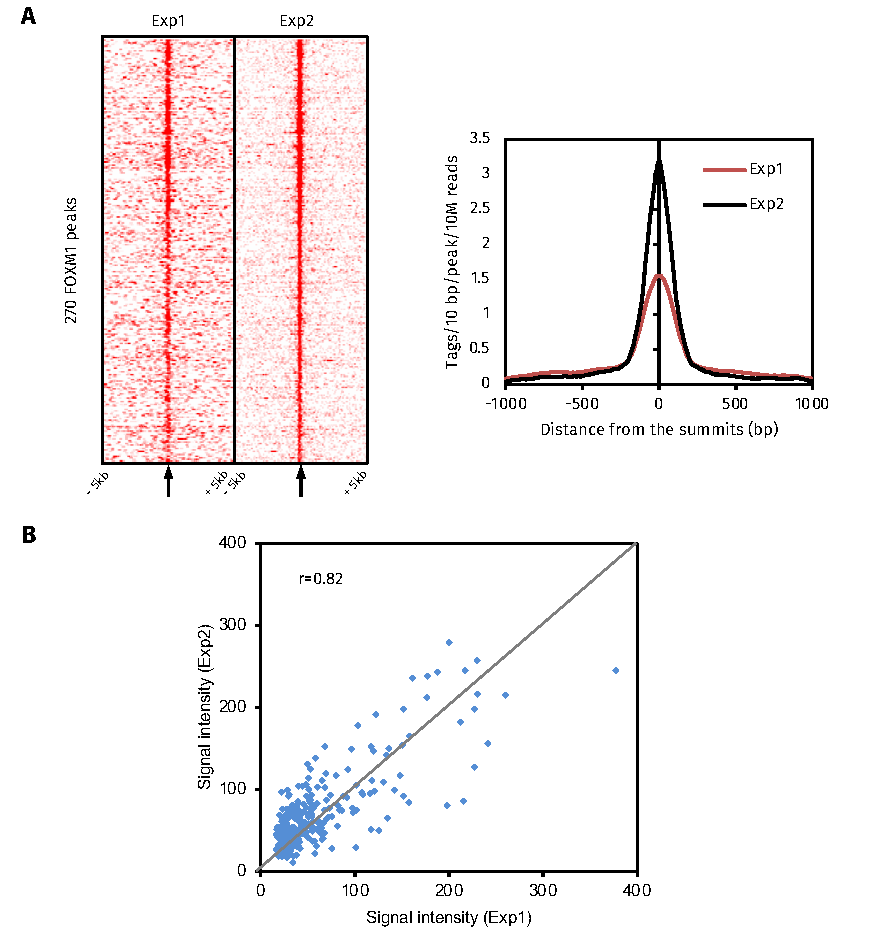
\includegraphics[width=0.9\textwidth]{chapter3/figures_overview/fig12.pdf}
    \caption[Comparison of the two replicates of FOXM1 ChIP-seq experiment]{\textbf{Comparison of the two replicates of FOXM1 ChIP-seq experiment. (A) Left,} heatmap of tag density profiles of the two replicates of FOXM1 ChIP-seq experiments around peaks that were identified from both replicates. Tags were calculated in every 50 bp bin, and the density profiles were normalised to tags per 10 million total reads per bin. The middle point of each panel (indicated by small arrows below) represents the summit of the peak. 5 kb upstream and 5 kb downstream around the summit were plotted. \textbf{Right,} quantification of average of tags around the summit of peaks. Peaks were aligned by their summits, and a region of -1 and +1 kb relative to the summit was selected. Tags were calculated in every 10 bp bin and normalised to tags per 10 million total reads per bin per peak. \textbf{(B)} Quantitative comparison of signal intensities of the two replicates of FOXM1 ChIP-seq experiments across 1-kb bins around the peaks. $r$, Pearson correlation coefficient.}
    \label{fig:fig12}
\end{figure}

Different transcription factors have different tendencies to bind to promoters, enhancers or gene bodies (reviewed in \cite{macquarrie2011genome-wide}). To find out whether FOXM1, FOXO3 and FOXK2 have similar tendencies to bind to the genomic regions, the distributions of FOXM1, FOXO3 and FOXK2 relative to the annotated transcription start sites (TSS) were analysed by the \textit{cis}-regulatory element annotation system (CEAS) (\cite{shin2009ceas:}). The genomic distributions of their peaks varied greatly. Here we define promoters as regions that are from the 5'-UTR to 1 kb upstream of the TSS. FOXM1 tends to bind promoter regions, with 73.7\% of its peaks in promoters (\textbf{Figure \ref{fig:fig13}B}), and FOXM1 peaks are significantly depleted at distal intergenic and intronic regions comparing to the genome background ($P$-values: $5.85 \times 10^{-21}$ and $1.09 \times 10^{-14}$, respectively, Fisher’s exact tests). This pattern of distribution is similar to transcription factors like ELK1 which also tends to bind proximal promoter regions (\cite{odrowaz2012elk1}). The distributions of FOXO3 and FOXK2 peaks were nearly identical, and they were in stark contrast to that of FOXM1 peaks. Only a small proportion (\textasciitilde 5\%) of FOXO3 and FOXK2 peaks reside in promoters, although this proportion is still more than the genome background (\textbf{Figure \ref{fig:fig13}B}). The majority of the peaks of both factors are located in distal intergenic and intronic regions, suggesting potential enhancer binding activity of these two factors (\textbf{Figure \ref{fig:fig13}B}). This is very similar to many other transcription factors like GATA-2 (\cite{linnemann2011genetic}), and other Forkhead transcription factors like FOXA1 (\cite{hurtado2011foxa1}), but varies from FOXM1 and ELK1.

\begin{figure}[!h]
    \centering
    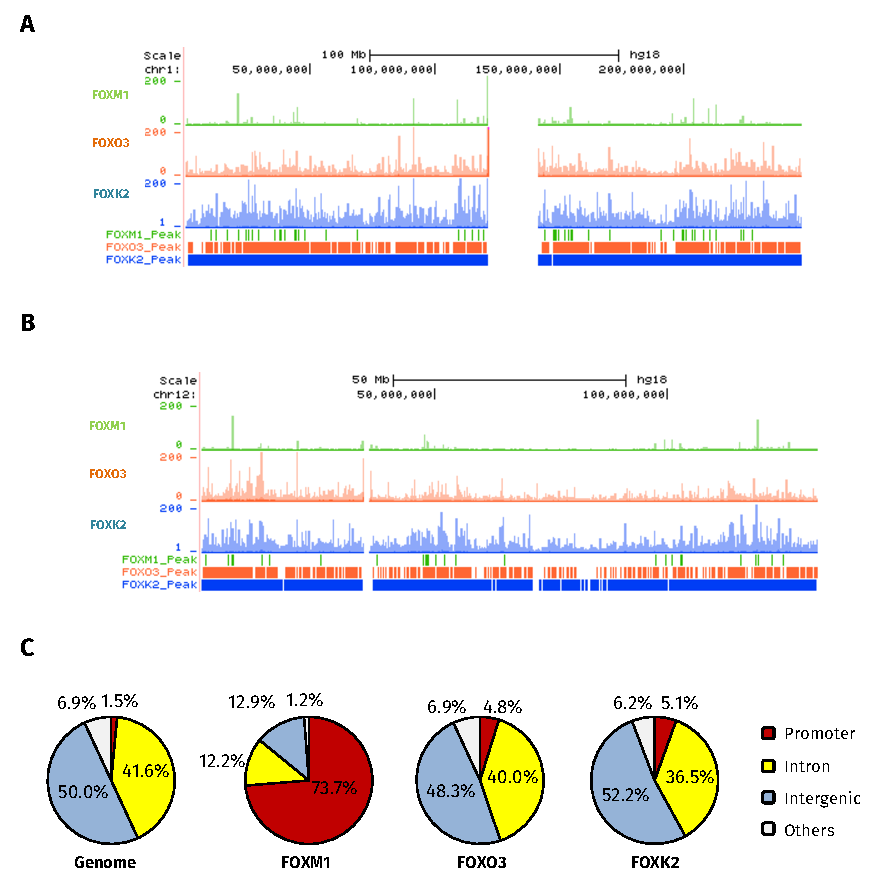
\includegraphics[width=0.9\textwidth]{chapter3/figures_overview/fig13.pdf}
    \caption[Examples of FOXM1, FOXO3 and FOXK2 ChIP-seq peaks]{\textbf{Examples of FOXM1, FOXO3 and FOXK2 ChIP-seq peaks. (A and B)} Two snapshots of all peaks for FOXM1, FOXO3 and FOXK2 on the entire chromosome 1 and 12. Locations of the peaks are indicated as bars (green for FOXM1, orange for FOXO3, and blue for FOXK2) below the peak profiles. Peak profiles on chromosome 1 is shown in \textbf{(A)}; peak profiles on chromosome 12 is shown in \textbf{(B)}. \textbf{(C)} The genomic distributions of the binding peaks for FOXM1, FOXO3 and FOXK2. Analyses were performed using \textit{cis}-regulatory element annotation system (CEAS). The promoter was defined as regions of 1 kb upstream from a transcription start site and the 5'-UTR. The distal intergenic region was defined as regions located 3 kb away from a gene body. Others were defined as regions including coding exon, 3'-UTR and up to 3 kb downstream from a transcription termination site. The distribution of genomic DNA is shown on the left.}
    \label{fig:fig13}
\end{figure}

Factors from the same family tend to have both redundant and specific binding events, due to their conserved DNA-binding domain. To investigate whether this is the case within FOXM1, FOXO3 and FOXK2, pairwise comparison of the peaks from the three Forkhead transcription factors were performed. Similar to members from other families, they had both overlapping and specific binding events (\textbf{Figure \ref{fig:fig14}A} and \textbf{B}). However, the extent of overlap among their peaks differed greatly. Here we define the overlapping peak as one where peaks share at least one base pair.

\begin{figure}[!h]
    \centering
    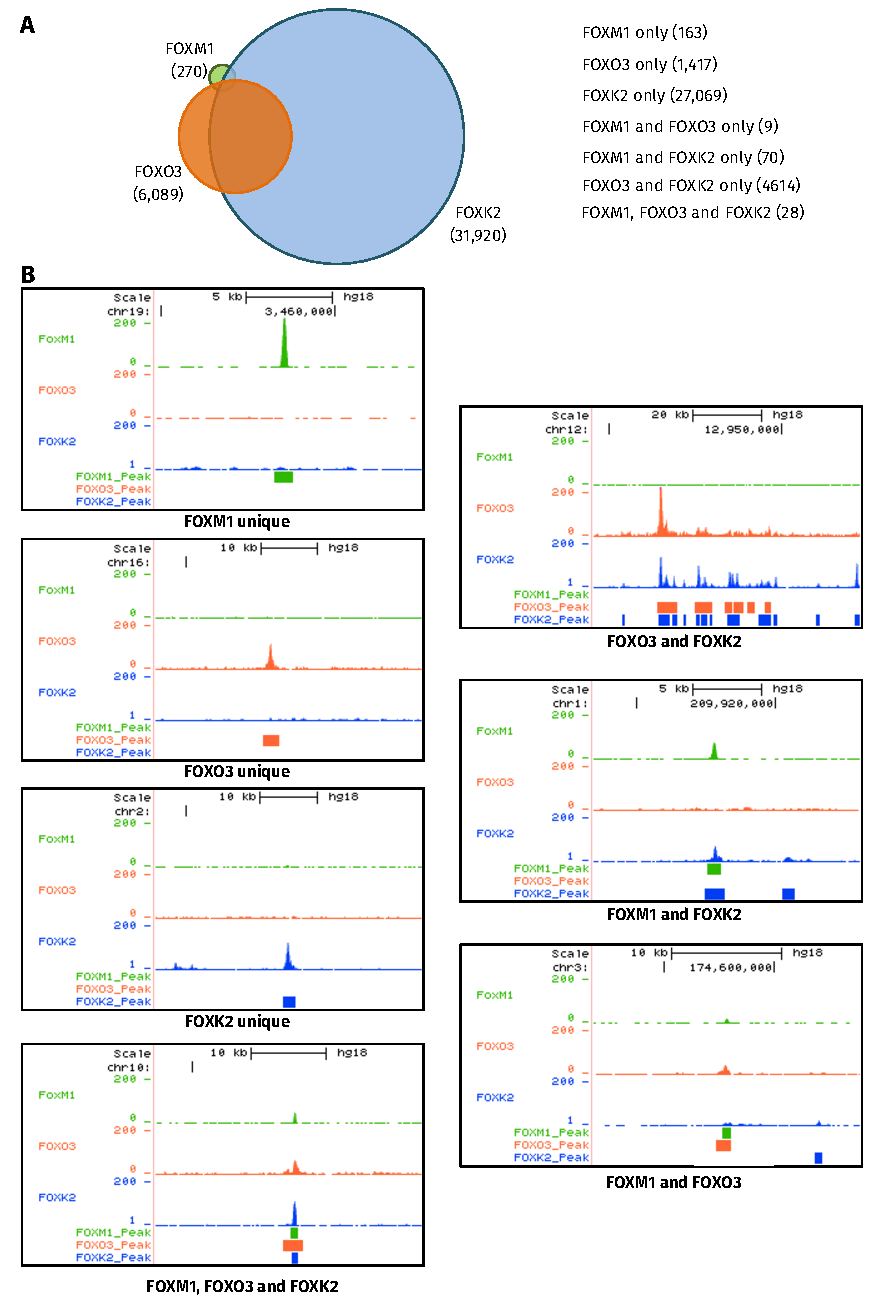
\includegraphics[width=0.8\textwidth]{chapter3/figures_overview/fig14.pdf}
    \caption[Examples of specific and overlapping binding events of FOXM1, FOXO3 and FOXK2]{\textbf{Examples of specific and overlapping binding events of FOXM1, FOXO3 and FOXK2. (A)} Venn diagram shows the overlap of the binding peaks for FOXM1, FOXO3 and FOXK2. \textbf{(B)} Snapshots showing examples of FOXM1, FOXO3 and FOXK2 peaks. Both unique and redundant peaks are shown.}
    \label{fig:fig14}
\end{figure}

Since FOXK2 had significantly more peaks than the other two factors, it also had many specific peaks of its own. However, the majority of FOXO3 peaks were shared with FOXK2 (\textbf{Figure \ref{fig:fig14}A}). Based on previous functional studies on FOXK2 and FOXO3 which suggest they have quite different biological functions (\cite{brunet1999akt,marais2010cell,ji2012the}), such a great level of overlap between FOXO3 and FOXK2 peaks is quite unexpected. For a more detailed analysis and discussion, see \textbf{Section \ref{section:foxo3}}).

Only 38 peaks were bound by both FOXM1 and FOXO3, and the FOXO3 binding signals around these 38 peaks were very low comparing to FOXM1, indicating the low occupancy of FOXO3 at these 38 peaks (\textbf{Figure \ref{fig:fig15}A}, left and middle panels). Furthermore, the FOXO3 binding signal was not located near the summits of FOXM1 peaks (\textbf{Figure \ref{fig:fig15}A}, left panel). In addition, when comparing the binding signals to the overall FOXO3 binding, it turned out that the FOXO3 binding at these 38 peaks were not as good as overall FOXO3 binding (\textbf{Figure \ref{fig:fig15}A}, right panel). Therefore, FOXM1 and FOXO3 do not seem to bind to the exact same regions.

There were 98 peaks shared by both FOXM1 and FOXK2. Although FOXK2 had decent binding signals around these 98 peaks, they were still very low compared to FOXM1 (\textbf{Figure \ref{fig:fig15}B}, left and middle panels). However, when comparing to the FOXK2 overall binding, the FOXK2 binding within these 98 peaks were comparable to its overall average binding signals (\textbf{Figure \ref{fig:fig15}B}, right panel). Indeed, we did observe higher signal intensities of FOXK2 in these 98 peaks comparing to the overall FOXK2 binding (\textbf{Figure \ref{fig:fig15}B}, right panel), but the background signals at these 98 peaks were also higher than the overall background, probably because most of these 98 peaks are located in core promoter regions which tend to get more reads in ChIP-seq experiments (\cite{auerbach2009mapping,cheung2011systematic}). In addition, the FOXK2 binding signals were also very close to the summits of FOXM1 peaks (\textbf{Figure \ref{fig:fig15}B}, right panel). Therefore, the position and the intensity of the FOXK2 signal profiles around these 98 peaks indicate that they represent binding regions for both FOXM1 and FOXK2.

\begin{figure}[!ht]
    \centering
    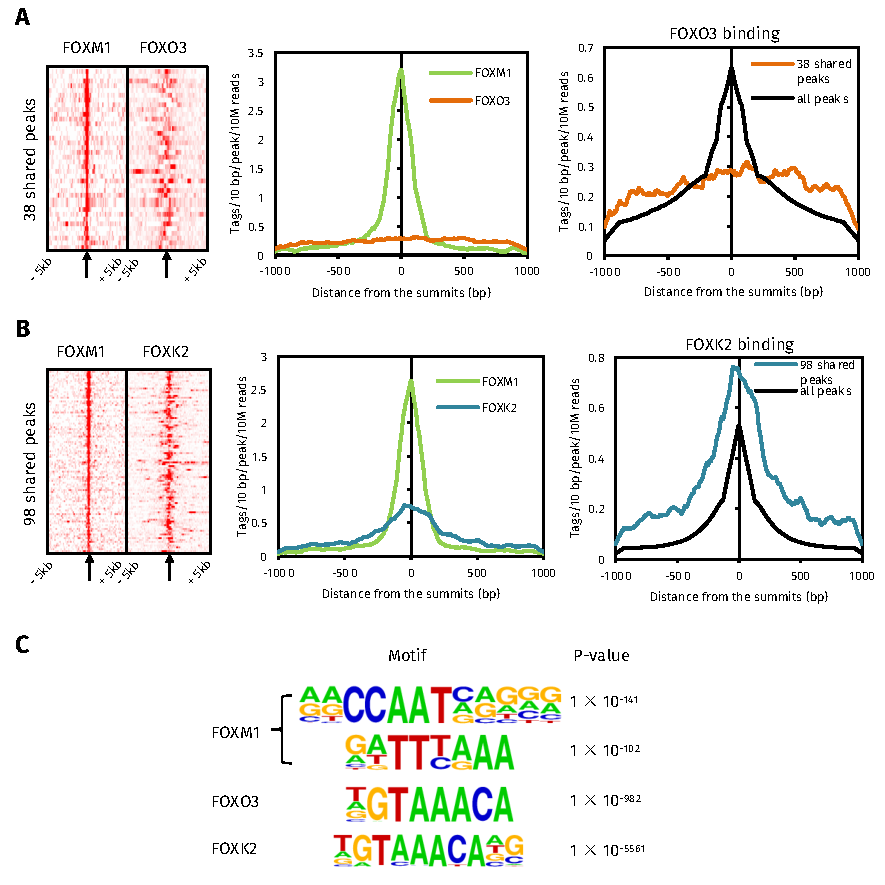
\includegraphics[width=0.8\textwidth]{chapter3/figures_overview/fig15.pdf}
    \caption[Comparisons of genome-wide binding events of Forkhead transcription factors]{\textbf{Comparisons of genome-wide binding events of Forkhead transcription factors. (A) Left,} heatmap of tag density profiles of FOXM1 and FOXO3 around the 38 peaks that are bound by both FOXM1 and FOXO3. Tags were calculated in every 50 bp bin, and the density profiles were normalised to tags per 10 million total reads per bin. The middle point of each panel (indicated by small arrows below) represents the summit of the FOXM1 peak. 5 kb upstream and 5 kb downstream around the summit were plotted. \textbf{Middle,} quantification of average of tags of FOXM1 and FOXO3 around the summit of the 38 peaks bound by both factors. Peaks were aligned by the FOXM1 summits, and a region of -1 and +1 kb relative to the summit was selected. Tags were calculated in every 10 bp bin and normalised to tags per 10 million total reads per bin per peak. \textbf{Right,} quantification of average of tags of FOXO3 on all FOXO3 peaks and the 38 peaks bound by FOXM1 and FOXO3. Tags were calculated in every 10 bp bin and normalised to tags per 10 million total reads per bin per peak. \textbf{(B)} The same analysis as \textbf{(A)} on the 98 peaks bound by both FOXM1 and FOXK2. \textbf{(C)} The top motifs returned by Homer \textit{de novo} motif discovery program from the 200 bp around the summits of ChIP-seq derived peaks for FOXM1, FOXO3 and FOXK2. The P-value was calculated based on hypergeometric distributions.}
    \label{fig:fig15}
\end{figure}

\textit{De novo} motif discovery is the most commonly-used method to find out the DNA sequence bound by a particular factor in the ChIP-seq study. The top motif returned by a motif discovery algorithm often reflects the DNA sequence bound by the factor \textit{in vivo}. To investigate the DNA sequences bound by these three Forkhead transcription factors, HOMER was used to perform \textit{de novo} motif discovery on the ChIP-seq data of FOXM1, FOXO3, and FOXK2. The most over-represented DNA sequence in the FOXM1 ChIP-seq peaks returned by HOMER were the CCAAT-box which is bound by the transcription factor NF-Y, and a motif that resembles the CHR (\underline{c}ell cycle \underline{h}omology \underline{r}egion) sequence (reviewed in \cite{müller2010the}). Surprisingly, the canonical Forkhead motif is not enriched in FOXM1 bound peaks (\textbf{Figure \ref{fig:fig15}C}). In contrast, the top DNA sequence motifs returned from the FOXK2 and FOXO3 ChIP-seq peaks were both canonical Forkhead motifs containing the core GTAAACA sequence (\textbf{Figure \ref{fig:fig15}C}).

In summary, FOXK2 has significantly more binding events than the other two Forkhead proteins. FOXO3 tends to bind redundantly with FOXK2, and only has a small proportion of specific peaks of its own. In contrast, FOXM1 seems to be an atypical Forkhead transcription factor and has its own specific binding event. This conclusion is based on its small number of peaks, its distinctive pattern of genomic distribution, the relatively low tag signals of FOXO3 or FOXK2 at peaks shared with FOXM1, and the completely different motifs enriched in its peaks.

\subsection{Summary}

Collectively, the data presented in this section provide a detailed description of the experimental strategies and general overviews of the ChIP-seq analyses of FOXM1, FOXO3 and FOXK2. The experiments are carefully designed in a factor-specific manner to obtain an optimal ChIP condition for each factor, and stringent criteria are used to get high confidence data. The initial comparison of the three ChIP-seq data sets reveals several surprising points.

The first surprising discovery is the number of binding sites of these three factors. The number of peaks identified for FOXK2, FOXO3, and FOXM1 varies greatly. FOXK2 and FOXO3 have a comparable number of binding events to other transcription factors. However, FOXM1 only possesses a small number of binding sites, which is significantly less than the number of peaks for other human transcription factors. This difference becomes even more conspicuous when comparing FOXM1 to other Forkhead transcription factors, which are generally believed to have a lot of binding sites \textit{in vivo} (\textbf{Table \ref{table:fkhtfschip}}).

\begin{longtable}{|c|c|c|c|}
    %% table setup %%
    \caption{Comparison of number of binding sites for different Forkhead TFs\label{table:fkhtfschip}}\\
    \hline
    \textbf{Forkhead Protein} & \textbf{Cell line} & \textbf{\# of binding sites} & \textbf{Reference}\\
    \hline
    \endfirsthead
    \multicolumn{3}{l}{\textbf{\textit{Table \ref{table:fkhtfschip}}} continued}\\
    \hline
    \textbf{Forkhead Protein} & \textbf{Cell line} & \textbf{\# of binding sites} & \textbf{Reference}\\
    \hline
    \endhead
    \hline
    \multicolumn{3}{l}{\textit{continued on the next page}}\\
    \endfoot
    \hline \hline
    \endlastfoot
    
    %% actual content %%
    FOXA1 & MCF7 & 79,651 & \cite{hurtado2011foxa1}\\
    \hline
    FOXA1 & T47D & 43,446 & \cite{hurtado2011foxa1}\\
    \hline
    FOXA1 & ZR75-1 & 80,327 & \cite{hurtado2011foxa1}\\
    \hline
    FOXA1 & HepG2 & 8,175 & \cite{motallebipour2009differential}\\
    \hline
    FOXA2 & HepG2 & 7,153 & \cite{motallebipour2009differential}\\
    \hline
    FOXA3 & HepG2 & 4,598 & \cite{motallebipour2009differential}\\
    \hline
    FOXH1 & H9 ESC & 9,702 & \cite{kim2011chromatin}\\
    \hline
    FOXK1 & HeLa & 4,329 & \cite{grant2012live-cell}\\
    \hline
    FOXK2 & U2OS & 31,920 & \cite{ji2012the}\\
    \hline
    \color{red} \textbf{FOXM1} & U2OS & \color{red} \textbf{270} & This study\\
    \hline
    FOXO3 & U2OS & 6,089 & This study\\
    \hline
    FOXP1 & H9 ESC & 3,400 & \cite{gabut2011an}\\
    \hline
    FOXP2 & PFSK-1 & 1,814 & ENCODE project\\
    \hline
    FOXP2 & SK-N-MC & 3,133 & ENCODE project\\
    \hline
    FOXP3 & MCF7 & 40,551 & \cite{katoh2011foxp3}\\
    \hline
\end{longtable}

The second surprising discovery is the genomic distribution of these three Forkhead transcription factors. The majority of both FOXO3 and FOXK2 peaks are located in the distal intergenic and intronic regions, and only a small proportion of their peaks reside in the promoter regions. This feature is commonly observed in other Forkhead transcription factors and indicates that FOXO3 and FOXK2 might be enhancer binding factors (\cite{wang2011reprogramming}).  However, most FOXM1 peaks are very close to the TSS and are depleted from the distal intergenic and intronic regions, which is in sharp contrast to FOXO3 and FOXK2 but similar to other transcription factors like ELK1 (\cite{odrowaz2012elk1}). This implies that the mechanism used by FOXM1 to regulate transcription is probably different from that used by FOXO3 and FOXK2.

The third, perhaps the most, surprising discovery is the enriched motifs within the peaks of these three factors. Forkhead-like responsive element containing the core GTAAACA and some motifs that resemble the binding sites of other transcription factors are enriched within the FOXO3 and FOXK2 peaks (see \textbf{Section \ref{section:foxo3}}), with the Forkhead motif being the most overrepresented motif in both cases. Only two motifs are found enriched within the FOXM1 peaks: one is the CCAAT-box motif which is bound by the transcription factor NF-Y; the other is the CHR motif which is bound by the DREAM and the MMB complexes. Furthermore, the Forkhead motif is not enriched within the FOXM1 cistrome.

Based on our preliminary analyses stated above, FOXM1 seems to somehow have its own specific binding events, while FOXO3 and FOXK2 are more like conventional members within the Forkhead family, which have both specific and overlapping binding sites. Therefore, in the following sections, we first analyse how FOXM1 obtains its own specific binding sites compared to other typical Forkhead transcription factors. Then FOXK2 and FOXO3 binding are compared to interrogate how they acquire their overlapping and specific binding events.